\section{Specific Requirements}

\subsection{External Interface Requirements}
The \textit{Travlendar+} application is a mobile based application.\\
In the following section, a more detailed description of the application is given, in terms of hardware, software and communication interfaces.\\
Are also given some basic prototypes of the User interface through mockups.
\subsubsection{User Interfaces}
Aiming at being as simple and intuitive as possible, the application has a UI which follows the principles of flat design.

\begin{itemize}
	\item \textbf{Logo}
	The logo of \textit{Travlendar+}, which will also be the logo icon for the app on smartphones, is minimal but elaborate at the same time.
	Multiple rounded rectangle and squares are combined in a way that makes possible to distinguish both the letter 't' and the symbol '+'. This logo will also be shown during the application opening phase. \\
	
	\begin{figure}[H]
		\centering
		
\includegraphics[width=0.17\textwidth]{logo_icon.png}
		\caption{Icon}
	\end{figure}

	\begin{figure}[H]
		\centering
		
\includegraphics[width=0.47\textwidth]{logo_inline.png}
		\caption{Logo}
	\end{figure}
	
	\newpage
	\item \textbf{Sign In/Sign up}\\
	This form is the first thing the User sees after opening the app. It allows the User to log in, signup or recover the password if lost. The registration module requires three mandatory fields..

	\begin{figure}[H]
		\centering
		\begin{subfigure}{0.25\textwidth}
			\centering
			
\includegraphics[width=\textwidth]{intro.png}
		\end{subfigure}
		~
		\begin{subfigure}{0.25\textwidth}
			\centering
			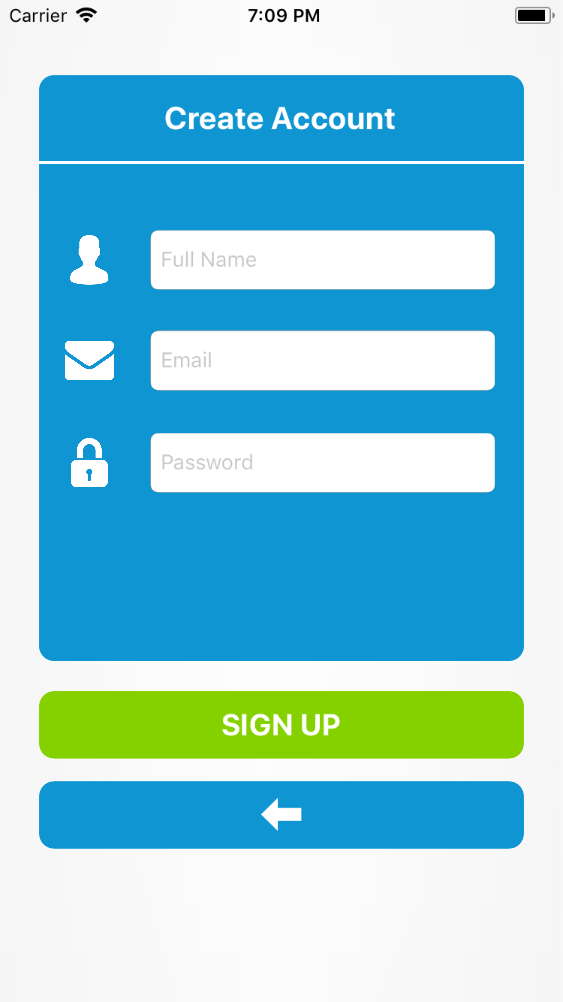
\includegraphics[width=\textwidth]{signup.png}
		\end{subfigure}
			~
	\begin{subfigure}{0.25\textwidth}
		\centering
		
\includegraphics[width=\textwidth]{confirmation.png}
	\end{subfigure}
	\caption{Sign in and sign up procedures}
	\end{figure}

	\item \textbf{Home page}\\
	Contains all the events of the current day, which could be expanded and edited, and a button to add a new event for the current day.
	 %each event in order to see all the information about the transportation means, the trip route and all the preferences. Moreover the User is allowed to add a new event during the day or edit one of the already existent.\\
	%The User is able to access to all the other pages.
	\begin{figure}[H]
		\centering
		\begin{subfigure}{0.25\textwidth}
			\centering
			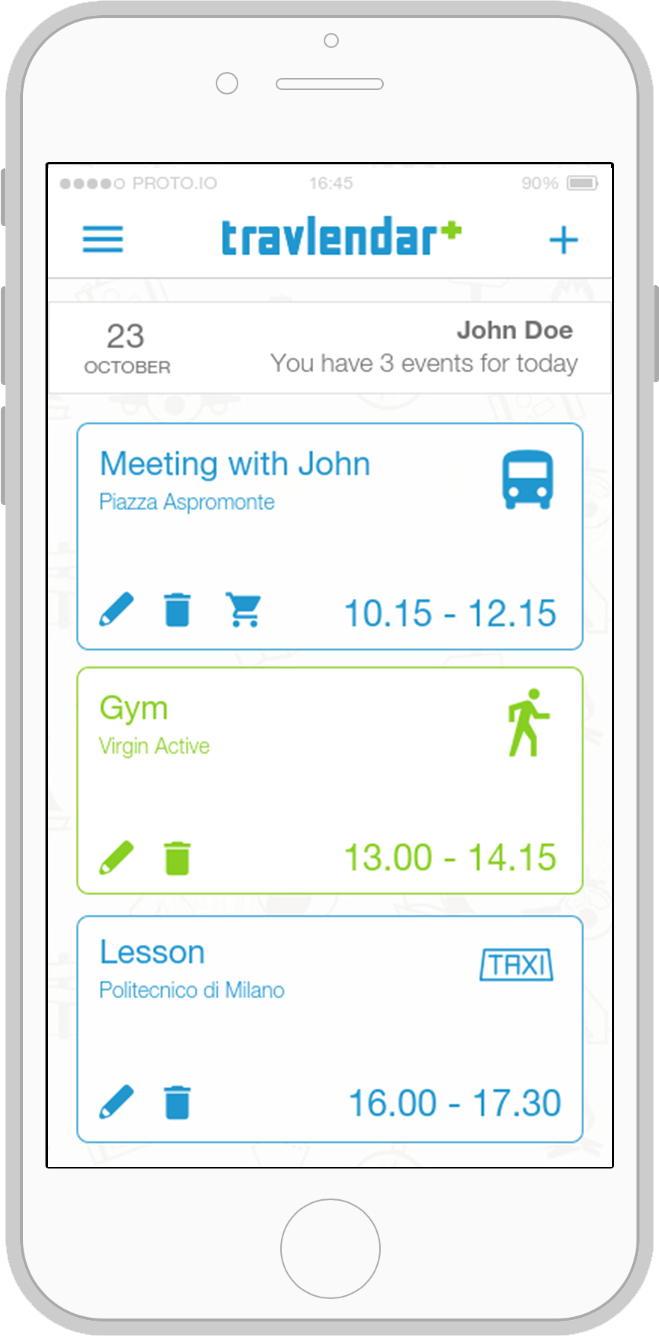
\includegraphics[width=\textwidth]{home_schedule.png}
		\end{subfigure}
	\caption{Daily schedule}
	\end{figure}

	\item \textbf{User settings}\\
	Used to view and edit the profile picture, personal email address, username and password.
	\begin{figure}[H]
	\centering
		\begin{subfigure}{0.25\textwidth}
		\centering
		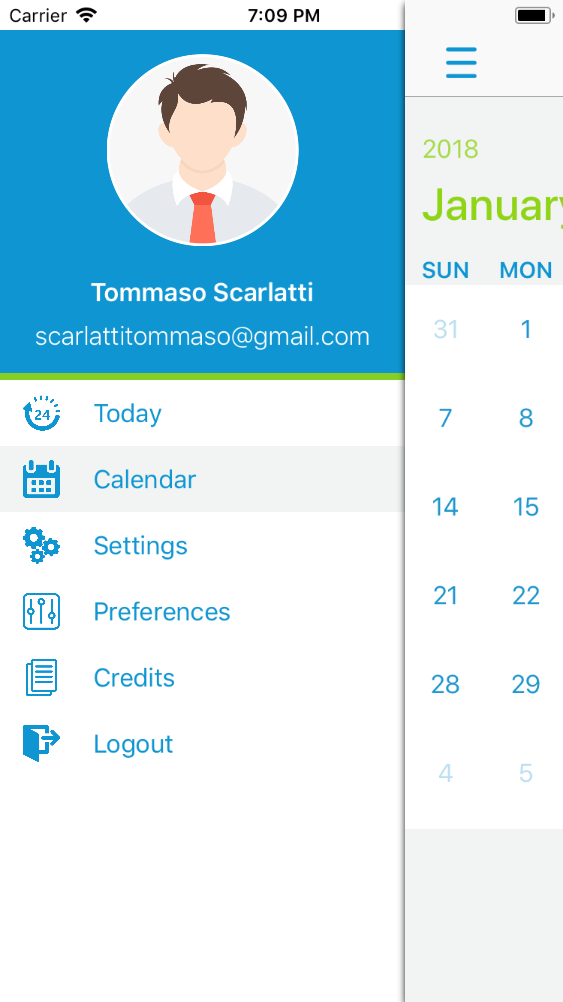
\includegraphics[width=\textwidth]{menu.png}
		\end{subfigure}
		~
		\begin{subfigure}{0.25\textwidth}
			\centering
			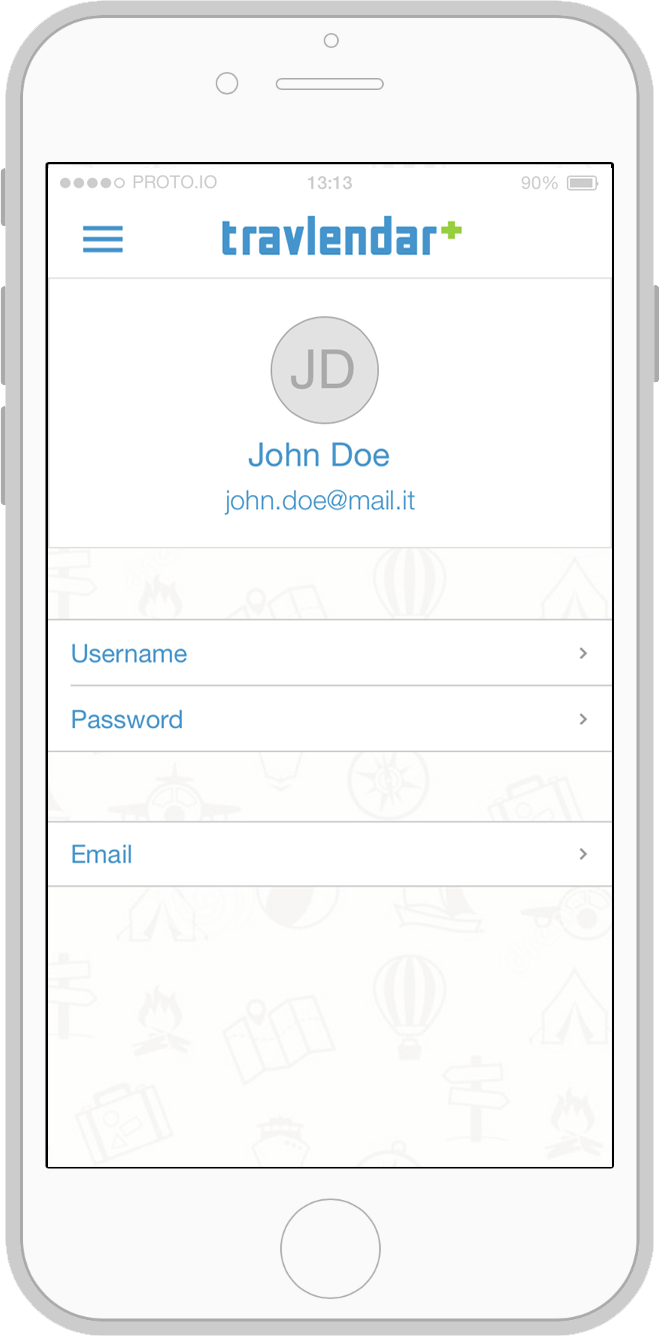
\includegraphics[width=\textwidth]{user_settings.png}
		\end{subfigure}

	\caption{Menu and User settings}
	\end{figure}

	\item \textbf{User preferences}\\
	In this page the User is able to activate or deactivate the available travel means and to set specific constraints for each of them.
	\begin{figure}[H]
		\centering
		\begin{subfigure}{0.25\textwidth}
			\centering
			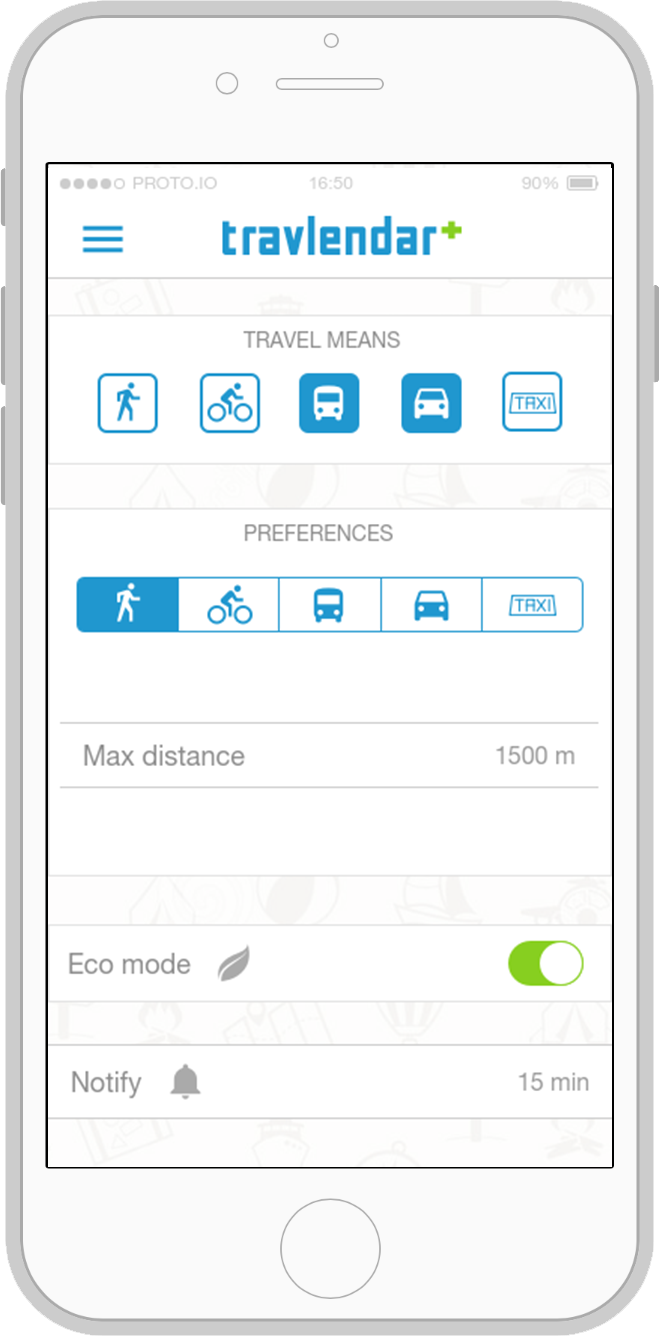
\includegraphics[width=\textwidth]{user_preferences.png}
		\end{subfigure}
		\caption{User preferences view}
	\end{figure}
	
	\item \textbf{Calendar page}\\
	Displays the  User calendar with a bullet for each day with at least one event scheduled. 
	\begin{figure}[H]
		\centering
		\begin{subfigure}{0.25\textwidth}
			\centering
			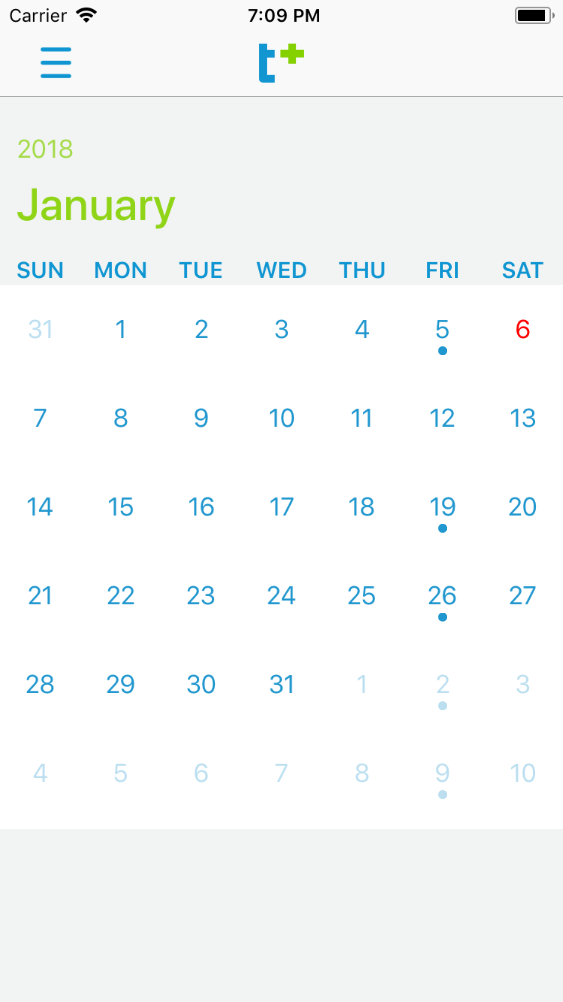
\includegraphics[width=\textwidth]{calendar.png}
		\end{subfigure}
		\caption{Calendar view}
	\end{figure}
		

	\item \textbf{New/Edit event}\\
	Opened when an User wants to add a new event to the calendar or to edit an existent one. If fields are consistent and there is no conflict in the schedule a list of possible travel options is shown.
	\begin{figure}[H]
		\centering
		\begin{subfigure}{0.25\textwidth}
			\centering
			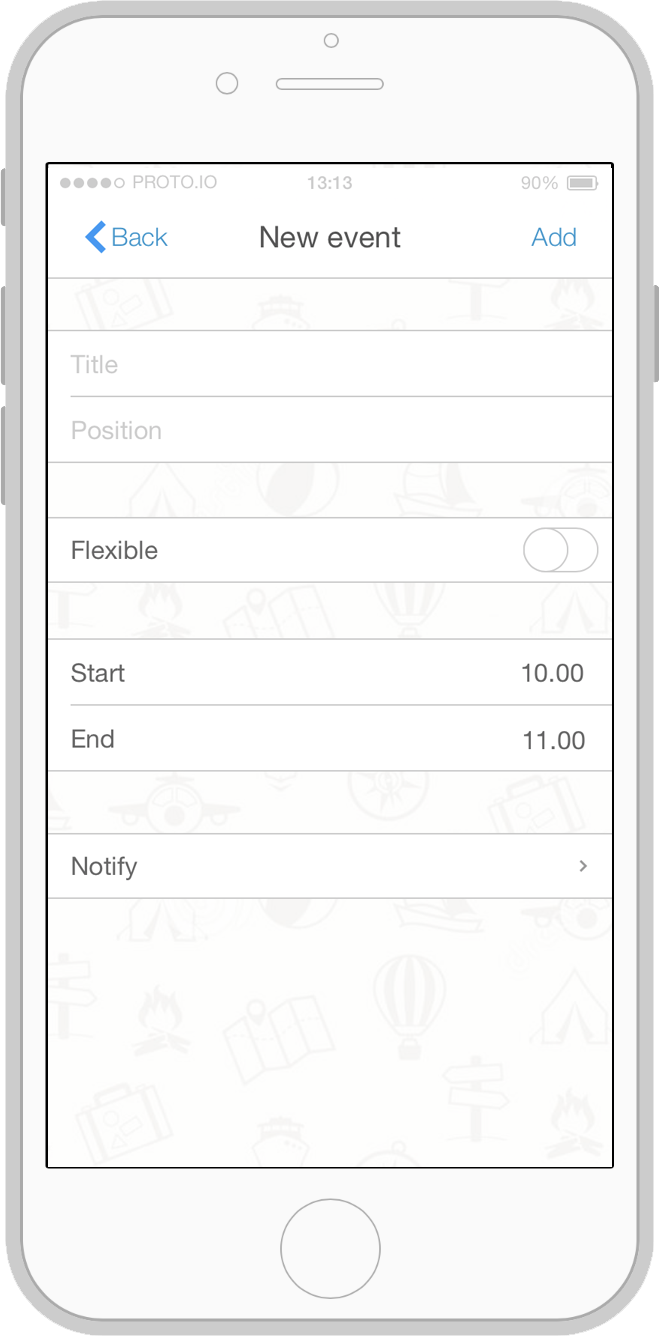
\includegraphics[width=\textwidth]{add_event.png}
		\end{subfigure}
		~
		\begin{subfigure}{0.25\textwidth}
			\centering
			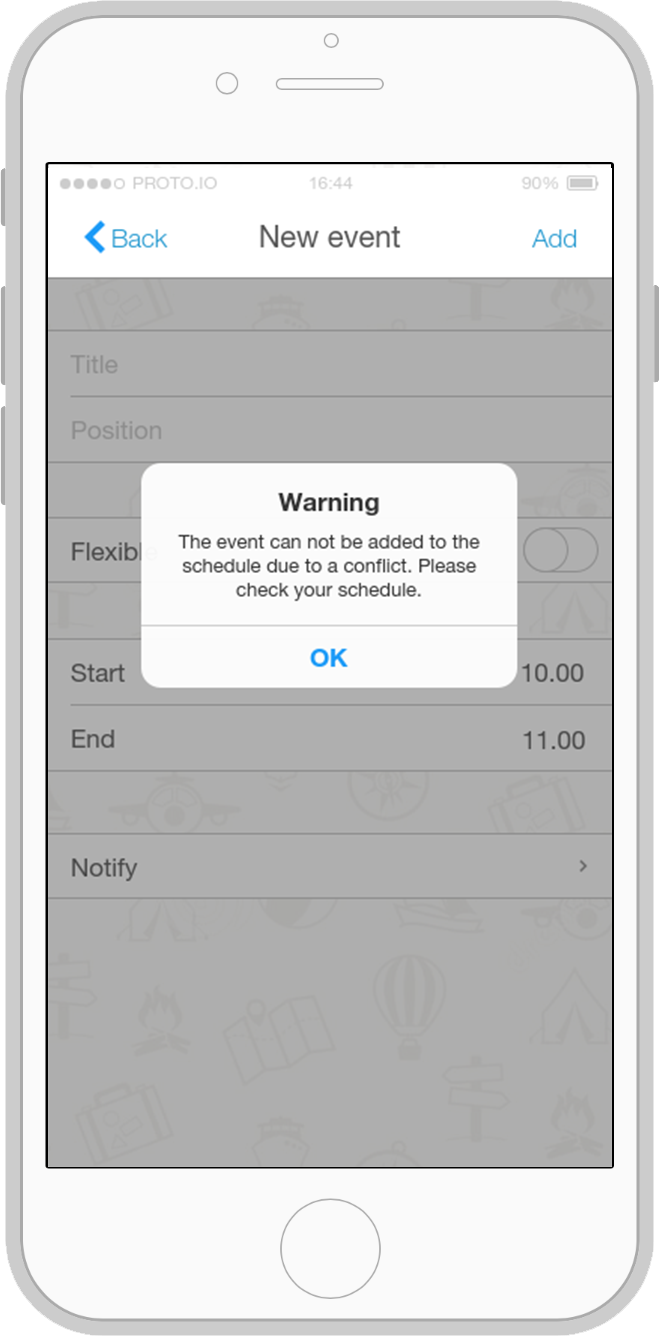
\includegraphics[width=\textwidth]{schedule_conflict.png}
		\end{subfigure}
		~
		\begin{subfigure}{0.25\textwidth}
			\centering
			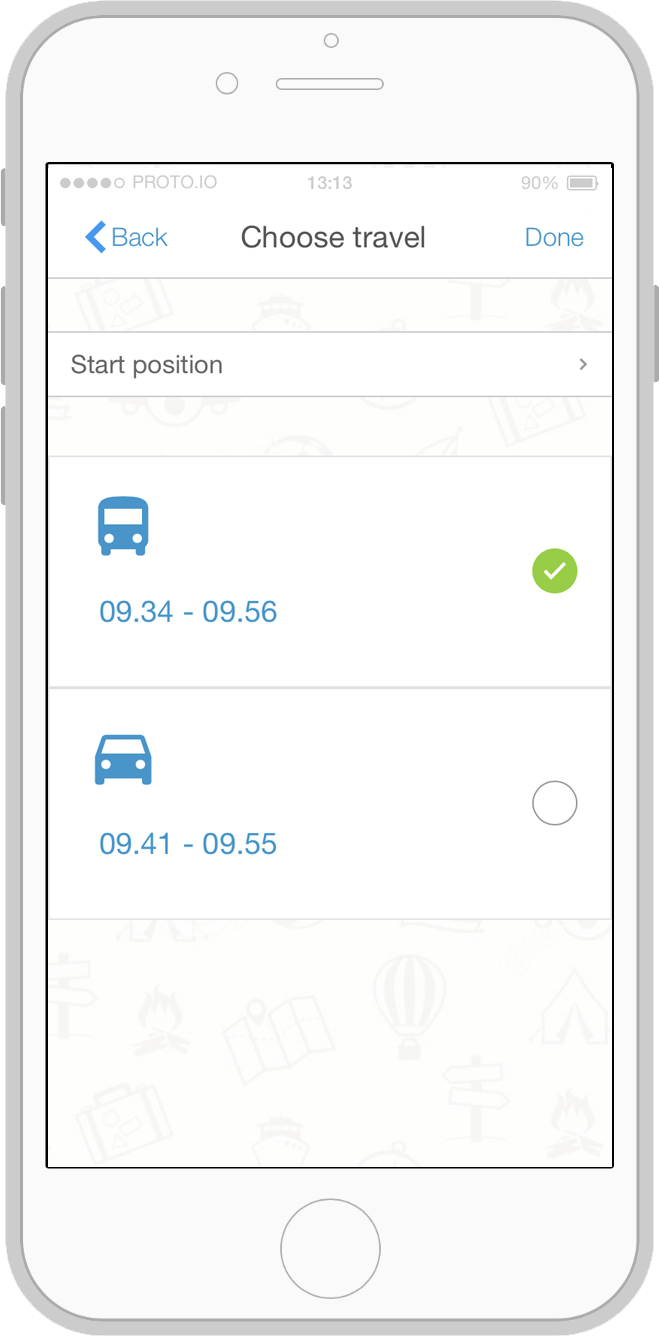
\includegraphics[width=\textwidth]{choose_travel.png}
		\end{subfigure}
	\caption{Add event procedure}
	\end{figure}
%	The User should be able to:
%	\begin{itemize}
%		\item Change the name of the event
%		\item Change the place of the event
%		\item Select the daytime of start and end of the event
%		\item Choose category of the event
%		\item Add a description of the event
%		\item Select the flexibility of the hour of the event: 
%		\item Select possibility for the notification: if is selected, the User should be able to chose when he wants to be notified
%		\item The means of transport selected by the User and the possibility for an "eco" transport
%	\end{itemize}

\end{itemize}
\subsubsection{Hardware Interfaces}
The application is available for mobile devices that guarantee Internet access. The web application can be accessed by any device that provides a reasonably recent browser.

\subsubsection{Software Interfaces}
\begin{itemize}
	\item Operating System: iOS, Android
	\item Web Browser
	\item Web Server application
	\item Development Frameworks
	\item DBMS
	\item Booking System: APIs for third party external services
	\item Mailing System: APIs to send emails to the User
	\item Mapping System: APIs for retrieve transport information
\end{itemize}

\subsubsection{Communication Interfaces}
The application will use HTTPS protocol for communication over the Internet and with the DBMS.

\subsection{Functional Requirements}
In the following section are explained the functional requirements of the application.
\begin{itemize}
	\item \textbf{[R.1]} A visitor must be able to register. During the registration the System will ask to provide credentials.
	\item \textbf{[R.2]} The System must check if the Guest credentials are valid: 
	\begin{itemize}
		\item the username is not already taken by another registered User
		\item the email is in the right format
		\item the password has a minimum length.
	\end{itemize} If credentials are correct, the System sends a confirmation email.
	\item \textbf{[R.3]} The System must store all User data such as personal information, credentials and schedule information.
	\item \textbf{[R.4]} The System must allow the User to log in using his/her personal credentials.
	\item \textbf{[R.5]} The System must allow the User to change username, only if the new username is not already in use by another User, email, only if the new email is in a correct format and password, only if the new password is different from the precedent and respects the minimum length.
	\item \textbf{[R.6]} The System must send a confirmation email if username, email or password is changed. The System must replace the old credentials with the new one.
	\item \textbf{[R.7]} The User must be allowed to create events, specifying:
	\begin{itemize}
		\item The name of the event
		\item The location of the event
		\item The location from which the event will be reached
		\item Start and end date of the event
		\item Start and end time of the event
		\item Notification option
	\end{itemize}
	\item \textbf{[R.8]} The User must be allowed to edit or delete a specific event in his/her schedule.
	\item \textbf{[R.9]} The System allows the User to provide optional event information. This informations are:
	\begin{itemize}
		\item Category type of the event
		\item Brief description of the event
	\end{itemize}
	\item \textbf{[R.10]} The System must allow the User to view all the events for a window of time.
	\item \textbf{[R.11]} The System must check if the event created or edited by the User is feasible.
	\item \textbf{[R.12]} The System must compute travel time between appointments.
	\item \textbf{[R.13]} The System must guarantee a feasible schedule, that is, the User is able to move from an appointment to another in time. The System must warn the User in case of unfeasible event preventing the creation. 
	\item \textbf{[R.14]} The System allows the User to add or edit an event only if it's not in conflict with other events already existent.
	\item \textbf{[R.15]} The System must allow the User to select a specific event.
	\item \textbf{[R.16]} The System must compute the best mobility options taking into account User preferences. If specified, the System must calculate the feasible combination of transportation that minimize carbon footprint.
	\item  \textbf{[R.17]} The System must allow the User to choose one of the mobility option during the event creation and the editing phase of the event.
	\item \textbf{[R.18]} The System allows the User to define specific constraint for each travel means, that are:
	\begin{itemize}
		\item The maximum distance reachable for each mobility option.
		\item The minimum distance of travel necessary for a specific mean of transport to be take into account.
	\end{itemize} 
	\item \textbf{[R.19]} The System must allow the User to be notified a specific time before any event.
	\item \textbf{[R.20]} The System must allow the User to select the \textit{Eco Mode} in order to minimize carbon footprint.
	\item \textbf{[R.21]} The System must allow the User to create flexible events and add additional informations that are:
	\begin{itemize}
		\item Time window in which the event could be created
		\item Duration of the event
	\end{itemize}
	\item \textbf{[R.22]} The System must allow the User to create repetitive events, adding information concerning:
	\begin{itemize}
		\item start/end time
		\item location of the event
		\item frequency of repetition.
	\end{itemize}
	\item \textbf{[R.23]} The System must check the feasibility of flexible events. The System must adapt these events in the schedule only if they are not in conflict with other events already in the schedule. 
	\item \textbf{[R.24]} The System must check the feasibility of repetitive events, taking into account an estimation of the travel time computed at the moment of the creation of the event.
	The System must warn the User in case of conflicts for some of the day specified: the User will be allowed to add the event only in the day with no conflicts or to discard the event creation.
	\item \textbf{[R.25]} For each occurrence of a repetitive event, the User will be allowed to request travel options and choose a travel mean.
	\item \textbf{[R.26]} The System must allow the User to select a specific travel means.
	\item \textbf{[R.27]} The System must provide an interface for third party services allowing the User to authenticate with the service.
	\item \textbf{[R.28]} The System must allow to activate notification and setting its time.
	\item \textbf{[R.29]} The System must activate a ring at the time selected by the User.
\end{itemize}

\subsection{Goals, Requirements and Domain Assumptions}
In the following section functional requirements and domain assumptions are grouped under each goal.
\begin{itemize}
	\item \textbf{[G.1] The System allows the User to access the functionalities of the application from different locations and devices. The data has to be coherent across different devices.}
	\begin{itemize}
		\item [] \textbf{Requirements}
		\item \textbf{[R.1]} A visitor must be able to register. During the registration the System will ask to provide credentials.
		\item \textbf{[R.2]} The System must check if the Guest credentials are valid: 
		\begin{itemize}
			\item the username is not already taken by another registered User
			\item the email is in the right format
			\item the password has a minimum length.
		\end{itemize} If credentials are correct, the System sends a confirmation email.
		\item \textbf{[R.3]} The System must store all User data such as personal information, credentials and schedule information.
		\item \textbf{[R.4]} The System must allow the User to log in using his/her personal credentials.
		\item \textbf{[R.5]} The System must allow the User to change username, only if the new username is not already in use by another User, email, only if the new email is in a correct format and password, only if the new password is different from the precedent and respects the minimum length.
		\item \textbf{[R.6]} The System must send a confirmation email if username, email or password is changed. The System must replace the old credentials with the new one.
		\item [] \textbf{Domain assumptions}
		\item \textbf{[D.1]} The given email is assumed to be correct.
		\item \textbf{[D.2]} The sent mail is assumed to be correctly received.
		\item \textbf{[D.3]} The Storage System is reliable.
	\end{itemize}

	\item \textbf{[G.2] The System allows the User to manage meetings in his/her schedule.}
	\begin{itemize}
		\item [] \textbf{Requirements}
		\item \textbf{[R.4]}The System must allow the User to log in using his/her personal credentials.
		\item \textbf{[R.7]} The User must be allowed to create events, specifying:
		\begin{itemize}
			\item The name of the event
			\item The location of the event
			\item The location from which the event will be reached
			\item Start and end date of the event
			\item Start and end time of the event
			\item Notification option
		\end{itemize}
		\item \textbf{[R.8]} The User must be allowed to edit or delete a specific event in his/her schedule.
		\item \textbf{[R.9]} The System allows the User to provide optional event information. This informations are:
		\begin{itemize}
			\item Category type of the event
			\item Brief description of the event
		\end{itemize}
		\item \textbf{[R.10]} The System must allow the User to view all the events for a window of time.
		\item \textbf{[R.11]} The System must check if the event created or edited by the User is feasible.
		\item [] \textbf{Domain assumptions}
		\item \textbf{[D.3]} The events informations provided by the user are correct.
	\end{itemize}

	\item \textbf{[G.3] The System allows the User to reach every meeting on time.}
	\begin{itemize}
		\item [] \textbf{Requirements}
		\item \textbf{[R.12]} The System must compute travel time between appointments.
		\item \textbf{[R.13]} The System must guarantee a feasible schedule, that is, the User is able to move from an appointment to another in time. The System must warn the User in case of unfeasible event preventing the creation. 
		\item \textbf{[R.14]} The System allows the User to add or edit an event only if it's not in conflict with other events already existent.
		\item [] \textbf{Domain assumptions}
		\item\textbf{[D.4]} Event time constraint are respected by the User.
		\item \textbf{[D.5]} The informations about the event are correct.
	\end{itemize}

	\item \textbf{[G.4] The System allows the User to select or edit a travel means to reach an event.}
	\begin{itemize}
		\item[] \textbf{Requirements}
		\item \textbf{[R.15]} The System must allow the User to select a specific event.
		\item \textbf{[R.16]} The System must compute the best mobility options taking into account User preferences. If specified, the System must calculate the feasible combination of transportation that minimize carbon footprint.
		\item  \textbf{[R.17]} The System must allow the User to choose one of the mobility option during the event creation and the editing phase of the event.
		\item[] \textbf{Domain assumptions}
		\item \textbf{[D.6]} The informations about available mobility options and related travel time are correct.
		\item \textbf{[D.7]} If selected, the private means of transport are available without any delay.
		\item \textbf{[D.8]} The start location of the travel is known and correct.
	\end{itemize} 

	\item \textbf{[G.5] The System allows the User to set preferences.}
	\begin{itemize}
		\item [] \textbf{Requirements}
		\item \textbf{[R.4]} The System must allow the User to login using his/her personal credentials.
		\item \textbf{[R.18]} The System allows the User to define specific constraint for each travel means, that are:
		\begin{itemize}
			\item The maximum distance reachable for each mobility option.
			\item The minimum distance of travel necessary for a specific mean of transport to be take into account.
		\end{itemize} 
		\item \textbf{[R.19]} The System must allow the User to be notified a specific time before any event.
		\item \textbf{[R.20]} The System must allow the User to select the \textit{Eco Mode} in order to minimize carbon footprint.
		\item [] \textbf{Domain assumption}
		\item \textbf{[D.9]} All selected travel means specified in the preferences are potentially available to the User.
		\item \textbf{[D.10]} A minimum walking distance is assumed in order to reach every mean of transport. Such distance will not be taken into account unless significant with respect to the travel time, meaning unless it influences the ETA by more than a minute.
	\end{itemize}

	\item \textbf{[G.6]} The System allows the User to create flexible events and repetitive events.
	\begin{itemize}
		\item [] \textbf{Requirements}
		\item \textbf{[R.4]} The System must allow the User to login using his/her personal credentials.
		\item \textbf{[R.21]} The System must allow the User to create flexible events and add additional informations that are:
		\begin{itemize}
			\item Time window in which the event could be created
			\item Duration of the event
		\end{itemize}
		\item \textbf{[R.22]} The System must allow the User to create repetitive events, adding information concerning:
		\begin{itemize}
			\item start/end time
			\item location of the event
			\item frequency of repetition.
		\end{itemize}
		\item \textbf{[R.23]} The System must check the feasibility of flexible events. The System must adapt these events in the schedule only if they are not in conflict with other events already in the schedule. 
		\item \textbf{[R.24]} The System must check the feasibility of repetitive events, taking into account an estimation of the travel time computed at the moment of the creation of the event.
		The System must warn the User in case of conflicts for some of the day specified: the User will be allowed to add the event only in the day with no conflicts or to discard the event creation.
		\item \textbf{[R.25]} For each occurrence of a repetitive event, the User will be allowed to request travel options and choose a travel mean.
		\item [] \textbf{Domain assumption}
		\item\textbf{[D.4]} Event time constraint are respected by the User.
	\end{itemize}

	\item \textbf{[G.7] The System allows the User to book transportation for a travel.}
	\begin{itemize}
		\item [] \textbf{Requirements}
		\item \textbf{[R.4]} The System must allow the User to login using his/her personal credentials.
		\item \textbf{[R.26]} The System must allow the User to select a specific travel means.
		\item \textbf{[R.27]} The System must provide an interface for third party services allowing the User to authenticate with the service.
		\item [] \textbf{Domain assumptions}
		\item \textbf{[D.11]} The User is registered to the service which offers the booking option.
	\end{itemize}

	\item \textbf{[G.8] The System allows the User to be notified before the occurrence of an event.}
	\begin{itemize}
		\item [] \textbf{Requirements}
		\item \textbf{[R.4]} The System must allow the User to login using his/her credentials.
		\item \textbf{[R.28]} The System must allow to activate notification and setting its time.
		\item \textbf{[R.29]} The System must activate a ring at the time selected by the User.
		\item [] \textbf{Domain assumptions}
		\item \textbf{[D.12]} The System internal clock time used to provide notifications is correct.
	\end{itemize}
\end{itemize}

\subsection{Performance Requirements}
\textit{Travlendar+} is structured in a three-tier architecture. All the application logic is built in the application servers: the backend performances should guarantee the proper operation in case of traffic peaks and manage multiple Users.

\subsection{Design Constraints}
\subsubsection{Standards Compliance}
All Informations concerning locations are given in form of Latitude and Longitude degrees. 

\subsubsection{Hardware Limitations}
The application should be able to run, at least, under the following conditions:
\begin{itemize}
	\item 3G connections at 2Mb/s
	\item 50 MB of space
	\item 2 GB of RAM
\end{itemize}

\subsection{Software Attributes}

\subsubsection{Reliability}
The System should guarantees a $99\%$ of reliability: its components must have a failure rate that guarantees this goal.

\subsubsection{Availability}
The System guarantees an high availability, due to the expected high reliability, in order to offer an ideal 24/7 service.

\subsubsection{Security}
User credentials and data will be stored in a DBMS that should guarantee an high security. For what concerns the User credential, in order to provide this result, the passwords stored in the DBMS are salted and hashed.\\
As already mentioned, the System uses HTTPS protocol to communicate with all the services, in order to guarantee protection of the privacy and integrity of the exchanged data.\\
The payment security for the booking functionality is guaranteed by third-party services and the System is not responsible in case of damage. 

\subsubsection{Maintainability}
The System will have a modular architecture: each component is organized in a hierarchical way in order to speed up the maintenance in case of failure. This structure is also convenient for further refinements of single components.

\subsubsection{Portability}
The application is developed in terms of Web Application and native application for iOS and Android. Furthermore, the three-tier architecture of the System allows to define a backend in which all the business logic is built, ensuring an high level of portability.

